\chapter{Knowledge Graphs}\label{chap:kgs}

\chapterQuote{\hfill\textit{``Knowledge is hot water on wool. It shrinks time and space.''}}{--- \textit{House of Leaves}, Mark Z. Danielewski}

\chapterAbstract{K}{nowledge Graphs (KGs) are ...}
how the chapter is structured

% are collections of facts that are represented in a graph-like structure, with entities and connections between them. This chapter provides an introduction to KGs, and it is structured as follows: Section~\ref{sec:kgs-intro} introduces the reader to their history and main characteristics. Section~\ref{sec:kgs-current} provides an overview of the most prominent KGs in use nowadays. Section~\ref{sec:kgs-applications} presents some of the many practical applications of Knowledge Graphs. Section~\ref{sec:kgs-challenges} reflects on the main current challenges regarding KGs. At last, Section~\ref{sec:kgs-summary} summarizes and concludes this chapter.

\section{Introduction}\label{sec:kgs-intro}
knowledge graphs are so cool blah blah blah...

% Representing and storing structured domain-specific knowledge has been an active research topic since at least 1970, when the first relational databases were introduced \cite{codd1970}. Given their indisputable success, many alternative means of representing knowledge in an structured manner have been proposed over the years. One of such proposals was using what was coined as a \textit{Knowledge Base} (KB) \cite{hayes-roth1983}, a collection of facts that are stored as direct relations between concepts. Contrary to relational databases, which need to go through a normalization process that introduces a number of indirections to represent a piece of knowledge, KBs were considered more straightforward to operate and reason about \cite{russell2020}. A number of Knowledge Bases were thus created and maintained throughout the subsequent years by multiple organizations and research entities, which were both general-purpose~\cite{mahdisoltani2014,lehmann2015dbpedia, rebele2016, carlson2010, bollacker2008, vrandevcic2014} and domain-specific~\cite{chakravarty2017, thorn2013pharmgkb, wishart2009, wishart2008, kanehisa2010}.

% The information inside a Knowledge Base was stored in the form of entities, which represented real-world or domain-specific concepts, and relations that link these entities together. This is known as a triple: a combination of two entities by means of a relation, which usually contains a verb. For example, a KB can represent the fact that Magnus Carlsen is a chess player using the triple \textit{(Magnus Carlsen, plays, Chess)}. Such triples were generally encoded in a KB using the RDF/XML format \cite{decker2000}, or an extension of it called RDFS, which allows for a higher degree of expressivity. However, since RDF/XML is mainly intended for machine use, later KBs also used other formats, like N3, Turtle, or RDF/JSON, which are more human-readable.

% However, the introduction of the Google Knowledge Graph in 2012 \cite{singhal2012} was a pivotal point for both the industrial use and academic research of Knowledge Bases. Rather than a simple collection of relations between names of entities, they started to be seen as a rich, interconnected structure of elements (\textit{``things, not strings''}) with an enormous potential for practical and commercial applications. Many other large companies of the likes of Amazon, Facebook, Microsoft and eBay soon followed suit \cite{shrivastava2017, krishnan2018, pittman2017, noy2019}, and the term Knowledge Graph (KG) rose to the popularity it still enjoys nowadays, replacing the denomination ``Knowledge Base''.

% In the following sections, we present the most popular Knowledge Graphs that are under active use today and the ways in which they are constructed. We then discuss the many practical applications that can, and have been, derived from the usage of KGs in commercial and academical contexts. However, despite their many benefits, Knowledge Graphs still present several challenges that must be addressed to improve their functionality and usefulness. Therefore, we also provide an overview of the main open challenges that need to be addressed to refine and improve Knowledge Graphs.

\section{Current Knowledge Graphs}\label{sec:kgs-current}
esta seccion la tenia agu para hablar de los grafos actuales, no la veo mal para comentar cuales se usan para investigacion y tal.

pero le cambiaria el nombre a Notable Examples o Modern KGs o algo del palo.

hablar de los que se han usado obv.


% Nowadays, there are a number of popular Knowledge Graphs under active use, either commercial or academical. Some of the most prominent ones are as follows:

% \begin{itemize}
%     \item \textbf{DBpedia \cite{lehmann2015dbpedia}:} Initially, the DBpedia project aimed to obtain a graph-like structure from semi-structured information sources, mainly, from the infoboxes present in Wikipedia articles (see Figure~\ref{fig:kgs-infobox}). Once this was achieved, DBpedia was further enhanced by adding links to external KGs and general open resources. DBpedia is both a multi-domain and multi-language KG, with a rich and publicly available ontology that enhances the contents in it. It also supports live synchronization with dynamic Wikipedia articles, to ensure that its knowledge is consistently up-to-date.
    
%     \begin{figure}[!htp]
%         \centering
%         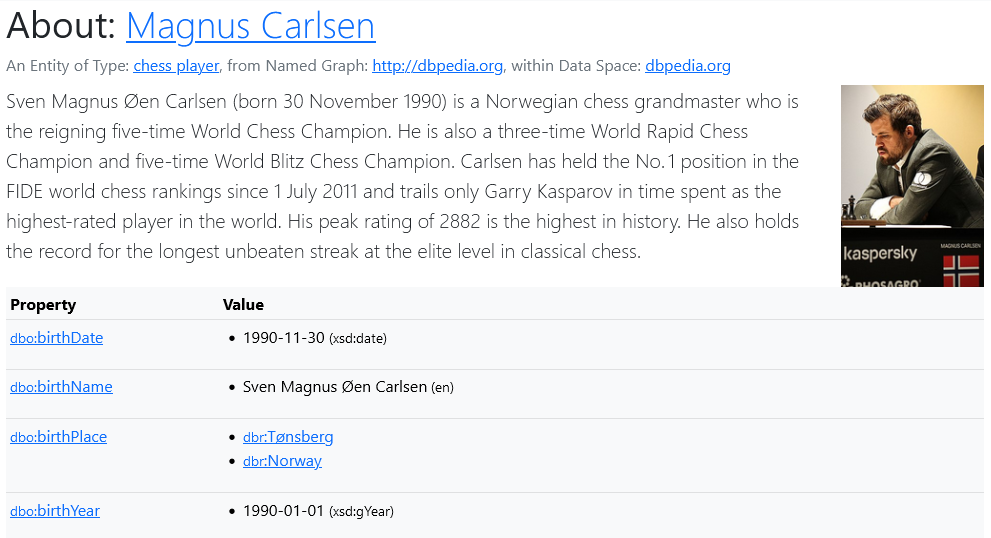
\includegraphics[width=\textwidth]{fig/kgs/dbpedia.png}
%         \caption{The entity \textit{Magnus Carlsen} in DBpedia}
%         \label{fig:kgs-dbpedia}
%     \end{figure}

%     \item \textbf{YAGO \cite{rebele2016}:} A Knowledge Graph that shares a number of similarities with DBpedia. Just like it, YAGO is also a KG that extracts semi-structured information from Wikipedia to create, as its authors put it, a \textit{``light-weight and extensible ontology with high quality and coverage''} \cite{suchanek2007}. A number of refinements are applied to the knowledge stored in YAGO, such as canonicalization, which removes possibly duplicate elements from the graph; or type checking, which prevents invalid combinations of entities from being formed.
    
%     \item \textbf{FreeBase \cite{bollacker2008}:} A large-scale, multi-domain KG that aimed to collect human knowledge in order to facilitate its integration, usage and standardization. Unlike the previously discussed KGs, which use Wikipedia as their main sources of information, FreeBase was a collaborative project that relied on human editors and curators to add knowledge to it. It was also one of the first multimodal KGs, since it allowed users to include text, images and media files. FreeBase was acquired by Google in 2010 and, upon the release of the Google Knowledge Graph, it was discontinued and put in a read-only mode. However, it is still a popular Knowledge Graph in the academic domain, since many different research works use it to benchmark their proposals.
    
%     \begin{figure}[!htp]
%         \centering
%         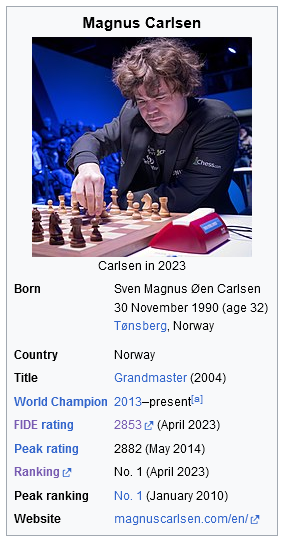
\includegraphics[width=.4\textwidth]{fig/kgs/infobox.png}
%         \caption{A Wikipedia infobox}
%         \label{fig:kgs-infobox}
%     \end{figure}

%     \item \textbf{WikiData \cite{vrandevcic2014}:} After KGs such as DBpedia and YAGO successfully leveraged the information in Wikipedia's infoboxes, the Wikimedia Foundation soon realized that the information contained in them could be very useful. However, the data in these boxes needed to be manually added, edited and updated by human editors, and constantly kept up-to-date in as many languages as the original articles were available in. To alleviate this issue, they introduced WikiData as a centralized and crowdsourced source of information, to supply Wikipedia articles and a number of other applications with data. Contrary to most other KGs, and following the philosophy of Wikipedia, all data entered into WikiData is not immediately considered a fact, but rather a claim that must be supported by references to outside sources. Both entities and relations in WikiData are denoted with codes, which makes it language-agnostic, but can reduce its human interpretability if they are not mapped to their human-readable names. Figure~\ref{fig:kgs-wikidata} shows a small excerpt of WikiData, centered around the entity \textit{Artist}.
    
%     \begin{figure}[!htp]
%         \centering
%         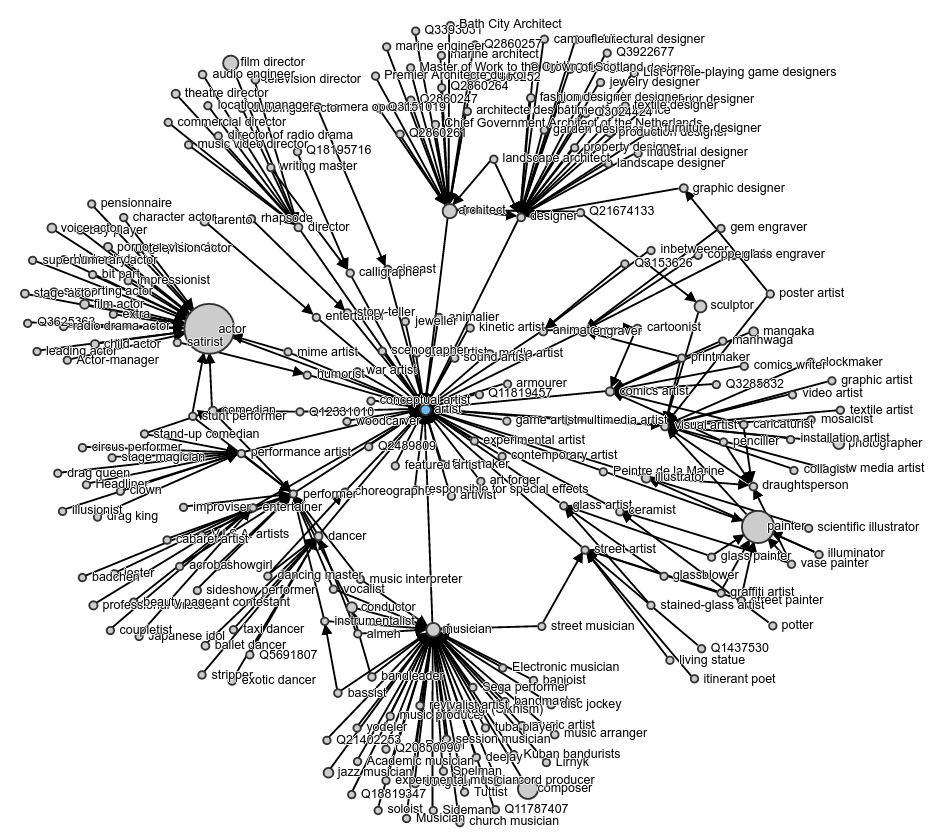
\includegraphics[width=\textwidth]{fig/kgs/wikidata.png}
%         \caption{An excerpt of WikiData}
%         \label{fig:kgs-wikidata}
%     \end{figure}
    
%     \item \textbf{NELL \cite{mitchell2018}:} The Never-Ending Language Learning project, or NELL for short, is a fully-automated system that scans the entire web, reads the contents of a webpage, and attempts to extract information from plain text written by humans. The information it extracts is then structured in the form of a triple and inserted in a KG. This Knowledge Graph is thus, by its very definition, under constant expansion. The NELL project allows users to rate an extracted fact positively or negatively, depending on whether or not the fact makes sense and is correct, and this allows the extractor to learn over time which facts are being successfully extracted, consistently improving its capabilities. NELL can also assign a confidence score to the facts it extracts, although only \textasciitilde6\% of its \textasciitilde50 million facts have a high confidence score.
    
%     \item \textbf{MAKG \cite{sinha2015}:} A prime example of a domain-specific KG, the Microsoft Academic Knowledge Graph is a very large collection of over 8 billion triples with meta-information about research, such as academic publications, authors, institutions, and domains of study, among others. The information in it is obtained directly from two main sources: academic publishers, such as ACM and IEEE, and websites indexed by the Bing search engine, from which the information must be extracted from a plain-text format. In total, more than 83 million papers and 20 million authors are present in this academic Knowledge Graph.

% \end{itemize}

\section{Applications}\label{sec:kgs-applications}

tambien una seccion obvia, tenemos que son, cuales hay y par que se usan, quizas alterar el orden y poner esta seccion antes de la anterior? hay pros y contras...

% It has been established that Knowledge Graphs are a powerful tool to organize and connect information in a semantically meaningful way, making it easier for machines and services to understand and interpret complex data. The use of Knowledge Graphs has expanded rapidly across a wide range of fields, including healthcare, education, e-commerce, and many others \cite{peng2023}. By providing a structured representation of data, Knowledge Graphs enable more accurate and efficient decision-making processes, support natural language processing, and enhance the ability of machines to understand the context and relationships between different entities. 

% In this way, Knowledge Graphs have proven to be an invaluable resource for a variety of practical applications that we take for granted nowadays, which require complex data management and analysis. Some of the most popular practical applications of Knowledge Graphs are as follows:

% \begin{itemize}
%     \item \textbf{Question answering:} Many search engines and personal assistants that are ubiquitous today, such as Siri, Alexa, Cortana, and Google Assistant, combine natural language processing (NLP) techniques, which helps them understand a query posed by a user, with Knowledge Graphs, which are used to navigate between entities and find the correct answer. Although most of the KGs that are used for this purpose are not made public for commercial reasons, they often contain a high amount of relations between both real-world and fictional entities and people. An example of this in practice is shown in Figure~\ref{fig:kgs-qa}.\\
    
%     \begin{figure}[!htp]
%         \centering
%         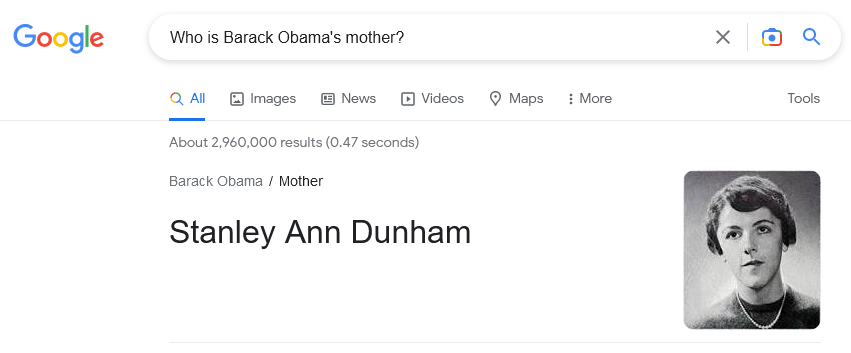
\includegraphics[width=\textwidth]{fig/kgs/qa.png}
%         \caption{Question answering using the Google Knowledge Graph}
%         \label{fig:kgs-qa}
%     \end{figure}

%     \item \textbf{Product recommendations:} Many authors \cite{zhang2021, palumbo2020, wang2019b, guo2022} have analyzed and proposed using Knowledge Graphs to issue product or media recommendations to users. By storing the relevant elements in a KG, such as the products that are on sale and the relations between them, and the users that bought or rated a product positively, one can apply a number of techniques to find a product that will be appealing to a new user in the system. The same concept can be applied for books or movies, a prime example of this is the movie information site IMDb, whose information has been used by Amazon to build a movie recommendation engine \cite{rele2022}.\newpage
    
%     \item \textbf{Advanced information retrieval:} Traditionally, information retrieval systems work by building and maintaining an index of a collection of documents and, when a user submits a query to the system, returns the documents that match the query more closely. However, this purely text-based approach falls short when it comes to semantical problems, for example, disambiguating an entity in the query, or interpreting it correctly. For this reason, some authors have proposed using Knowledge Graphs to enhance this process: for example, during the recent COVID-19 outbreak, \citet{wise2020} introduced a COVID-19 KG that aggregated the most recently published scientific works regarding this disease. This KG could be queried to quickly retrieve relevant research efforts, facilitating a worldwide collaboration to quell the pandemic.\\
    
%     \item \textbf{Education:} Multiple KG-centered proposals have been made in recent years to aid in several aspects of education. For example, \citet{chen2018} presented KnowEdu, a tool made for the purpose of building Knowledge Graphs out of educational materials. It is able to extract the main concepts of a subject or course, and then builds relations between them according to the activities and evaluation activities that the students will have to carry out in the future. \citet{aliyu2020} proposed building a KG containing the teachers, courses and scientific literature for a university, and using it to recommend relevant courses and books to students.\\
    
%     \item \textbf{Research:} Besides the previously discussed MAKG, a number of other Knowledge Graphs of research and academic entities have been built to help researchers explore possible lines of investigation and find possible relevant related materials. AceKG, introduced by \citet{wang2018}, is a similar KG, containing more than 3 billion triples with information about authors, papers, venues, and so on. The Artificial Intelligence KG \cite{dessi2020aikg}, and its extension, the Computer Science KG \cite{dessi2022cskg}, also contain a large volume of information pertaining research concepts, materials, tasks, and other similar entities in these fields. Furthermore, \citet{angioni2021} introduced the Academia/Industry KG, to help researchers identify trends in the constant exchanges between these two realms.\\
    
%     \item \textbf{Healthcare:} It is undoubtable that having an efficient and effective healthcare system is a cornerstone of a functional modern society. To help manage the ever-growing amount of medical data and records that healthcare professionals have to deal with, some proposals to integrate KGs in this field have been made. \citet{zhang2020b} presented HKGB, a KG builder aimed towards healthcare professionals that leverages their expertise to construct medical Knowledge Graphs. \citet{gong2021} proposed constructing KGs with information about medicines, diseases and patients, in order to use it to suggest medicines to patients with particular incompatibilities or intolerances. 
% \end{itemize}

\section{Open challenges}\label{sec:kgs-challenges}
The original subsections for this section was:
\begin{itemize}
    \item Integration
    \item Correction
    \item Completion
\end{itemize}

a more relevant subset for this paper could be:

\begin{itemize}
    \item Integration - knowwing which entities represent the same thing.
    \item Completion - adding missing links which are implicit.
    \item Reasoning - explainability to the new knowledge found.
\end{itemize}

as all of them are relevant for the topic.

offer special interest to completion and reasoning as they are more interesting towards the work presented.

% Despite the fact that Knowledge Graphs are already a well-established concept in research and industry, a number of challenges about their use and refinement still remain \cite{paulheim2017, hogan2020, peng2023}. In the following subsections, we delve into some of the most prominent ones in more detail. 

% \subsection{Integration}
% It is common that more than one Knowledge Graph contain information about the same real-world concept or entity. While each individual KG may include different additional information complementing it, it would be desirable that said information be integrated together, so as to have a single source of truth that contains a more comprehensive set of facts. The process of joining two or more Knowledge Graphs together is known as KG integration or fusion.

% The most challenging step of this process is determining which entities in different KGs refer to the same one in the real world, a task known as entity alignment \cite{ren2022}. Although this has been a very active research topic, some future directions can still be further explored. For example, it is still not clear how this can be done reliably when the KGs to be integrated have different languages, which could be useful for multilingual recommendation systems or question answering \cite{javed2021}. An attempt in this regard has been made by \citet{xu2019} using neural networks, however, the alignment accuracy they obtain is still not high enough to perform this process reliably.

% Moreover, most KG fusion approaches assume that the Knowledge Graphs to be fused together are of the same modality. This falls short in the presence of multi-modal KGs, for example, the previously discussed FreeBase. Joining together two or more KGs which entities can be represented in different formats is still an open challenge, although some authors have made recent proposals. \citet{guo2021} have presented HMEA, a multi-modal entity alignment technique by using hyperbolic spaces. \citet{cheng2022} proposed MultiJAF, a framework for multi-modal entity alignment. Despite this, the wide array of possible modalities that could be represented through a KG make multi-modal alignment a very challenging and still unsolved task.

% Furthermore, a related problem is entity disambiguation. This problem presents itself during the process of building the KG, and consists in determining the specific meaning of an entity written in natural text in the presence of ambiguity. For example, contextual information is required to determine whether \textit{``Armstrong''} refers to the astronaut, the jazz musician, or the cyclist. If this is not solved correctly, even a successful entity alignment can be poisoned by the fact that the entities that were aligned were not disambiguated properly upon their creation, and thus do not actually refer to the same concepts.

% \subsection{Correction}
% The previous analysis of the most popular Knowledge Graphs shows that automatic construction is the most common way to build a KG, due to the sheer amount of facts that they are intended to contain. It is therefore inevitable that these automated methods introduce a certain degree of incorrect information in the KG, either because it was not correctly interpreted, or because the original source of information was wrong.

% Refining a KG after its creation by detecting wrong facts is known as Knowledge Graph correction. The most common way to perform this task is to do fact validation \cite{paulheim2017}, which assigns a confidence score in the interval $[0, 1]$ to every triple in the KG. Then, the triples that do not meet a minimum confidence threshold are purged from the graph.

% There exist a number of research works in the literature that propose different ways to do fact validation. \citet{pasternack2010} propose converting the facts in a KG into natural language sentences, and then using more general methods for fact checking. The same authors \cite{pasternack2011} also propose an alternative method, which groups up similar facts in a KG that provide support for each other, and then joins these groups to create more general justifications for the possible correctness of a fact. \citet{gerber2015} have proposed using classifiers, which can learn which facts are wrong by using a number of features. Of course, this requires that a manually-annotated set of correct and wrong triples is provided, which can be an arduous task. Another classification-based approach is proposed by \citet{syed2018}, in this case, based on textual evidence.

% A more refined ---and challenging--- approach to KG correction is to not only detect which facts are wrong, but to amend them if possible so that they represent correct knowledge. This is known as fact repairing. Due to the increased difficulty of the task, a smaller body of work can be found in the literature. \citet{topper2012} proposed leveraging the ontology of a Knowledge Graph to detect and fix inconsistencies in triples where the domain or range restrictions of the relation are violated, however, their proposal requires a human to step in and select the correct version of it out of the suggestions provided by the system. \citet{bonatti2011} proposed a fully-automated method for fixing triples, but it requires provenance and trust annotations to be present in the KG, which are relatively rare.

% \subsection{Completion}
% As previously discussed, most KGs are commonly built by extracting non-structured or semi-structured information from web sources, though some KGs can be manually curated by domain experts. When information extraction systems are applied to extract knowledge from online sources, that information is then semantized~\cite{ayala2018, neumaier2016} and stored in a KG as triples in the KG. Regardless of the specific process by which a KG is constructed, the resulting graph usually lacks a certain amount of information, either because said information was not originally present in the information source, or because it was unsuccessfully extracted or semantized~\cite{bordes2014b}. 

% Because of this inherent incompleteness, KGs operate under the Open World Assumption, i.e., a piece of information that is not present in a KG is not considered to be incorrect, but rather just unknown~\cite{galarraga2015}. Therefore, it is mandatory to refine KGs after their creation in order to expand the knowledge they contain~\cite{paulheim2017}.

% Deriving additional knowledge from an existing KG with the goal to augment it is a task known as Knowledge Graph completion~\cite{paulheim2017, shen2022overview}. In KG completion, the goal is to identify triples that are missing from the KG and have a chance of being correct that is as high as possible. To achieve this goal, a series of steps are usually carried out, which are visually depicted in Figure~\ref{fig:kgc-workflow}.

% \begin{figure}[!htp]
%     \centering
%     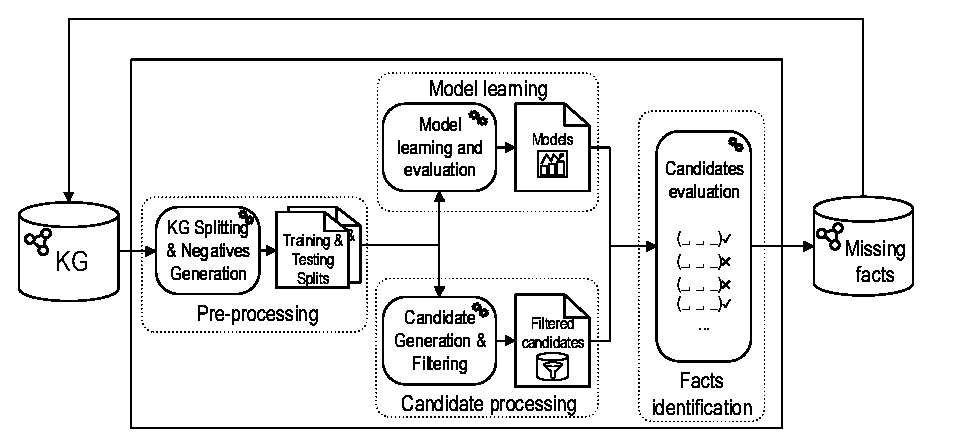
\includegraphics[width=\textwidth]{fig/kgs/kgc_workflow}
%     \caption{Knowledge Graph completion workflow}
%     \label{fig:kgc-workflow}
% \end{figure}

% First, the Knowledge Graph must be pre-processed in order to add negative triples, in the case they are not present, and split them between a training and a testing set \cite{ayala2019}. Then, a KG completion model is trained and evaluated using the sets of triples generated in the previous step. In parallel, a set of plausible candidate triples is materialized. If the KG completion model yields a satisfactory efficacy after its evaluation, it is applied on the candidate triples, to identify which ones are correct and which ones should be discarded \cite{borrego2021, borrego2019,shen2022overview}. Finally, the triples considered correct are added back to the Knowledge Graph, enriching it.

% In opposition to the previous two challenges, which focus on information that is already present in the graph, KG completion, by definition, focuses on finding knowledge that is not yet present. For this reason, it is particularly hard, and a number of authors have made different proposals to tackle it. Since the focus of this dissertation is on Knowledge Graph completion, the following chapters provide a more in-depth analysis of the existing proposals in the scientific literature to complete Knowledge Graphs.

\section{Summary}\label{sec:kgs-summary}
% This chapter has introduced the reader to Knowledge Graphs. It has provided a brief summary of their history and main characteristics, as well as a summary of the most prominent KGs that can be found today. Furthermore, it has presented the reader with an ample repertoire of practical applications of Knowledge Graphs, many of which we use in our daily lives. Finally, it has introduced some of the challenges regarding KGs that still remain open to this day, namely: Knowledge Graph integration, correction, and completion.

a brief summary of all topics in this chapter.
